\documentclass[dvipdfm,cjk,14pt,hyperref={bookmarks=false,compress,slidestop}]{beamer}
\AtBeginDvi{\special{pdf:tounicode EUC-UCS2}}
\renewcommand{\kanjifamilydefault}{\mgdefault}
\renewcommand{\baselinestretch}{1.4}
\usefonttheme{professionalfonts}
\usetheme{GrayGradient}
\usepackage[T1]{fontenc}
\usepackage[utf8]{inputenc}
\usepackage{lmodern}
\usepackage[sc]{mathpazo}
\usepackage[scaled]{helvet}
\usepackage[scaled]{beramono}
\usepackage[deluxe,expert]{otf}
\usepackage{textcomp,okumacro}
\usepackage{url}
\author{金子達哉 \texttt{(id:catatsuy)}}
\title{}
\date{}
\begin{document}

\begin{frame}
 \titlepage
\end{frame}

\begin{frame}
 \frametitle{自己紹介}
 \begin{itemize}
  \item 金子達哉
  \item はてな ID: \texttt{catatsuy}
  \item twitter: \texttt{catatsuy}
 \end{itemize}

\begin{picture}(0,0)(0,0)
 \put(200,0){
\includegraphics[clip, height=35truemm]{catatsuy}}
\end{picture}
 \vspace{-5pt}
 URL:
 \begin{itemize}
  \item \url{http://www.catatsuy.org}
  \item \url{http://blog.catatsuy.org}
  \item \url{https://matw.co}
 \end{itemize}
\end{frame}

\begin{frame}
 \frametitle{所属}
 \begin{itemize}
  \item 東京工業大学
  \item 情報工学科 4 年(9 月卒業予定)
  \item 吉瀬研究室\\
        \begin{itemize}
         \item コンピュータアーキテクチャ
        \end{itemize}
 \end{itemize}
\end{frame}

\begin{frame}
 \frametitle{就職活動}
 \begin{itemize}
  \item はてなインターン 2012
  \item pixiv インターン
 \end{itemize}
 \vspace{-20pt}
 \begin{center}
  \begin{tabular}{cc}
   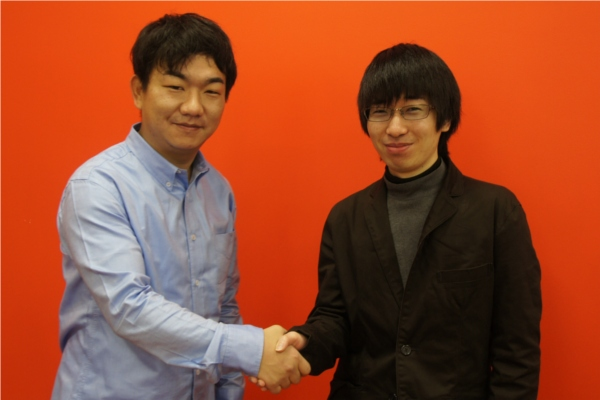
\includegraphics[clip, height=38truemm]{pixiv} & 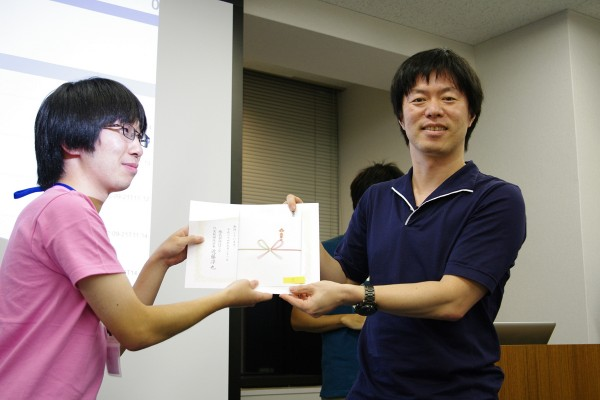
\includegraphics[clip, height=38truemm]{hatena} \\ 
  \end{tabular}
 \end{center}
\end{frame}

\begin{frame}[plain]
 \begin{center}
  \LARGE ド真ん中で叫ぶ
 \end{center}
\end{frame}

\begin{frame}[containsverbatim]
 \frametitle{verb 環境}

\begin{verbatim}
#include <stdio.h>
int main() {
  printf("hello, world\n");
  return 0;
}
\end{verbatim}

\end{frame}


\end{document}
